\subsubsection{Objects and Types}

All the visible graphical elements on the screens~\ref{img:screens} are the result of components that have been drawn into an HTML5 canvas element. Components are JavaScript objects specifically create within the kernel. While the functional programming style seems well suited for the task of evaluating the source files as I will show in a moment, a more classical object oriented approach better suits the purpose of maintaining a hierarchy of components that can share similar pieces of code with other components. They are objects in the sense of object oriented programing, with methods, fields and they can inherit from other components. Figure~\ref{img:componentsUML} shows a diagram over the components used in the sample application and what component they inherit from. They all inherit from the Base component which I have defined in my implementation as being abstract, meaning that it cannot be directly instantiated. It has no draw method! All components maintain their own dictionary of properties and list of children. 

Deep inside the kernel, within the canvas sub-module in \texttt{kernel/src/canvas.js} a simple JavaScript object is used as a dictionary to hold a registry over all the available type of components. There, the key --that represents the type name-- relates to a configuration object that is used when instantiating\footnote{In JavaScript, objects are not instantiated from classes, they are rather created using maker~\cite{crockford_inheritance} functions. When using the term instantiation in the context of JavaScript programing I usually refer to the action of calling such a maker function in order to create an object.} that type.

\begin{figure}
    \centering
    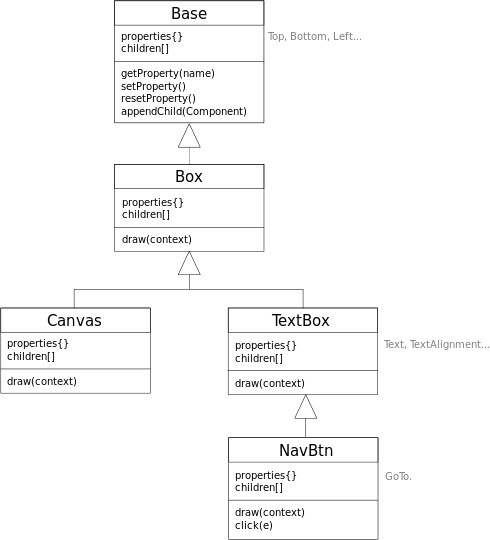
\includegraphics[width=0.9\textwidth]{images/components_uml.jpg}
    \caption{Component hierarchy}
    \label{img:componentsUML}
\end{figure}

\lstinputlisting[
    caption={The component maker function},
    label={lst:makeComponent}
]{code/makeComponent.js}

\paragraph{Instantiating a component} immediately causes the maker function to lookup the requested type in the dictionary of types. Then, based on the retrieved configuration object, a prototype\footnote{In JavaScript all objects have a prototype. The prototype can be either a reference to another object or the value null. When looking for a property on an object, if not directly found on that object, JavaScript will try to find the property on the object's prototype. It will keep following the prototype chain until it finds the value or meets the value null.} is created by looking at what type it should extend. The Base component does not extend any other type so it's prototype simply refers to \texttt{Object.prototype}. The simplicity behind simulating inheritance using the prototype chain is very exiting and powerful. As you can see in listing~\ref{lst:makeComponent}, the prototype of a component can potentially be a chain of component's since the maker function is invoked recursively. In this way, the hierarchical structure in diagram~\ref{img:componentsUML} is made possible. The component of type NavBtn will have TextBox as it's protoype which will have Box as it's prototype wich will have Base as it's prototype. When calling the method getProperty on NavBtn, JavaScript will lookup the prototype chain and finally find that method on the Base type.

When the prototype chain for a component is ready, the component is finally created using the fairly new JavaScript method \texttt{Object.create}. Each component has it's own set of properties and list of children. When the component is actually created, all the properties declared in the configuration object are \emph{cloned} into a new property. I insist on the word \emph{clone}. In JavaScript, objects are passed around by reference. A simple copy of a property object directly into the properties of the component to instantiate would have the dramatic consequence of having all component instances sharing a reference to the same object. Concretely, it means that if changing, let's say the value of the property Top on the component instance \texttt{x} this would also affect instances \texttt{y}, \texttt{z} and so on\dots. This needs to be absolutely avoided. Therefore the \texttt{createProperty} function ensures to create a new property with the name and the value registered on that properties configuration.

All other properties are simply copied from the configuration object to the properties of the component instance. This allows to copy and to eventually overrride the custom methods defined for a specific type. The maker function finally returns the new instance.

Based on this maker function principle~\ref{lst:makeComponent} it would be possible to also enable multiple inheritance, allowing thereby a component to inherit from more than a single component. This is particularly useful for GUI components.

\lstinputlisting[
    caption={Procedure for registering a new component},
    label={lst:registerComponentType}
]{code/canvas/registerComponentType.js}

\paragraph{The registration of a new type} of component is easy. It is a simple matter of adding the configuration object --that is used when instantiating that type-- into the dictionary of types. This configuration object must be validated in order to make sure that it contains at least an InitialValue and a Validator. We also want to make sure that it does not specify it's own type name as the type to extend, we don't want the type to be abstract if the configuration doesn't explicitly require so and finally we want to make sure that the InitialValue value passed the function associated to the Validator field. listing~\ref{lst:registerComponentType}

\paragraph{The validator} is a concept meant to simulate type checking when trying to assign a value to a component's property. We need to be sure that the a value can be used by the internal methods of a component. Prior to the assignment, the validator function is called with the value. What the validator does depends on it's type. Currently the validator types that I created do throw an error when the given value does not match the specified rules. A better implementation could eventually try to ``cast'' the value into another type. For instance, trying to transform a date into a meaningful number. When looking at the reference diagram~\ref{img:refDiagram} it appears visibly that the dates of the activities are evaluated into numbers used to position the components on the screen. I believe that the validator could operate such a transformation if it was also access to some kind of context.

\paragraph{New validator types can be registered} into the kernel similarly to how new component types are registered. An object is used as a dictionary to internally keep track on the existing validators.

\lstinputlisting[
    caption={Configuration object of the Base component},
    label={lst:registerBase}
]{code/canvas/registerBase.js}

\todo[inline]{explain how to register components and validators externally}

Now that we know what components are, what validators are and that we know that components have properties, that new components can be registered an so on, we can have a look at how the base component is registered. This is a special type of component since all other components inherits from it. The configuration object for that type is shown in listing~\ref{lst:registerBase} declares a getProperty method that is important to understand.

As it's name indicates the getProperty method returns a component property with a given name (if such a property exists). All components have their own local list of properties. The prototype of a component (the component it extends) also has a local list of properties and so on, all the way up through the prototype chain. When a component extends another one, it should inherit all of it's properties. If a component type specifies a new property, that property is local to the component and can be found in the local list of properties, otherwise it should be looked up in the properties of each component in the prototype chain. This is precisely what the getProperty method does. It tries to find the property locally to the current component, if unsuccessful, it recursively looks up the prototype chain. Finally it throws an Error if the property was not found. Note here that, because we treat the getProperty as a method of a component, the execution context of that function is bound to that component. The keyword \texttt{this} represents the current object. When calling the getProperty method recursively, for each invocation, the execution context must to be bound to the prototype, otherwise \texttt{this} will refer to the component the first invocation was made from. Within the getProperty method, each recursive call to itself explicitly binds the execution context of that function to the prototype to explore: \texttt{this.getProperty.call(prototype, name)}.

\subsubsection{Drawing the objects into a HTML5 Canvas}

\lstinputlisting[
    caption={Draw method},
    label={lst:draw}
]{code/canvas/draw.js}

All components extending the type Box will inherit from it's draw method, given that they don't override it by explicitly defining one in the type's configuration object. That method~\ref{lst:draw} uses the values of it's different properties in order to draw shapes into a context. The context is actually stored as a global variable within the canvas module and can be accessed from anywhere. However it is obviously passed to the draw function as an input parameter because external component types do not have access to that global variable, yet they must be able to implement their own draw method using the very same context. They would not have access to it otherwise. The context is defined when creating the HTML5 Canvas element for the first time, it is shipped by the element and offers the necessary tools for drawing advanced graphics on a web page.

Components that needs to extend or give a complete new behaviour to the draw method can do so by declaring their own draw method as a property in the configuration object when registering the new type. This is what the component of type TextBox does for instance. TextBox uses the same behaviour as what is defined in the draw method of a Box. But in addition to this, it adds a layer of text on to of it. This is done by accessing the prototype of TextBox (which is a Box) and by invoking it's own draw method: \texttt{const prototype = Object.getPrototypeOf(this); prototype.draw(context);}

The component of type Canvas is special. Beyond drawing using the context, it also changes the HTML Canvas element itself by setting some of it's properties (width, height). It also extends the type Box. It uses it's draw method in order to draw a background rectangle using the value of it's own backgroundColor property. The Type Canvas is abstract because a designer must not be able to instantiate it. It is only instantiated once by the kernel, in order to create to the top element of the instance tree, the tree that contains all the other components that must be drawn.

\subsubsection{Other important methods}

\lstinputlisting[
    caption={Reflow causes the entire tree of components to be drawn},
    label={lst:reflow}
]{code/canvas/reflow.js}

A function named reflow that is also available in the canvas module is shown here in listing~\ref{lst:reflow}. When called, it causes the entire tree of components to be drawn. Before drawing, it groups the components by looking their ZIndex property which allows the designer to redefine the default level at which the elements are rendered. The reflow will start calling the draw methods of all components starting by those with the smallest ZIndex, resulting in the components with a higher ZIndex being drawn on top of the other ones. Invoking a reflow is a costly operation and we therefore want to minimize that.

\lstinputlisting[
    caption={Inspect, a utility method that allows to reflect the existence of a component type and it's properties},
    label={lst:inspect}
]{code/canvas/inspect.js}

Finally, the canvas contains another important method called ``inspect''. In short, it allows to reflect the existence of a component type and it's properties. The method can take three parameters:
\begin{itemize}
    \item ``internal'' - a boolean value that is used to catch early in the compilation process if the designer addressed an abstract component type. This will throw an error.
    \item ``type'' - The name of a component type. The function checks if that name binds to a type configuration object in the dictionary of components.
    \item ``property'' - Optionally, the name of a component property. If provided, this third argument will be used to reflect the existence of a certain property on the given component type.
\end{itemize}
If a component type or a property on a component type does not exist the method returns \texttt{undefined}. The method is shown in listing~\ref{lst:inspect}.

By discussing the components, the validators and more generally the canvas module in the kernel, I have introduced the concepts used to enable the drawing of shapes similar to those used on the various screens~\ref{img:screens}. I have shown how to enable the local developer to support the designer by extending the built-in objects from his domain application. 

However, components are never directly instantiated by the designer nor by the local developer. They are instantiated by the kernel, through the specification of templates, built on the basis of actions taken by the designer and whose textual representation is stored in the vis file. In the next section I will discuss the evaluation process. It is an important part for producing the screens~\ref{img:screens} seen in our sample application. I will particularly focus on the screens relating to the ``Small dataset'' and ``bigger dataset'' menu entry. They make use of the most interesting capabilities of VisTool.